%%%%%%%%%%%%%%%%%%%%%%%%%%%%%%%%%%%%%%%%%
% Lachaise Assignment
% LaTeX Template
% Version 1.0 (26/6/2018)
%
% This template originates from:
% http://www.LaTeXTemplates.com
%
% Authors:
% Marion Lachaise & François Févotte
% Vel (vel@LaTeXTemplates.com)
%
% License:
% CC BY-NC-SA 3.0 (http://creativecommons.org/licenses/by-nc-sa/3.0/)
% 
%%%%%%%%%%%%%%%%%%%%%%%%%%%%%%%%%%%%%%%%%

%----------------------------------------------------------------------------------------
%	PACKAGES AND OTHER DOCUMENT CONFIGURATIONS
%----------------------------------------------------------------------------------------

\documentclass{article}

%%%%%%%%%%%%%%%%%%%%%%%%%%%%%%%%%%%%%%%%%
% Lachaise Assignment
% Structure Specification File
% Version 1.0 (26/6/2018)
%
% This template originates from:
% http://www.LaTeXTemplates.com
%
% Authors:
% Marion Lachaise & François Févotte
% Vel (vel@LaTeXTemplates.com)
%
% License:
% CC BY-NC-SA 3.0 (http://creativecommons.org/licenses/by-nc-sa/3.0/)
% 
%%%%%%%%%%%%%%%%%%%%%%%%%%%%%%%%%%%%%%%%%

%----------------------------------------------------------------------------------------
%	PACKAGES AND OTHER DOCUMENT CONFIGURATIONS
%----------------------------------------------------------------------------------------

\usepackage{amsmath,amsfonts,stmaryrd,amssymb} % Math packages

\usepackage{enumerate} % Custom item numbers for enumerations
\usepackage{longtable} % To display tables on several pages
\usepackage{rotating}
\usepackage[ruled]{algorithm2e} % Algorithms
\usepackage[spanish]{babel}
\usepackage[framemethod=tikz]{mdframed} % Allows defining custom boxed/framed environments

\usepackage{listings} % File listings, with syntax highlighting
\lstset{
	basicstyle=\ttfamily, % Typeset listings in monospace font
}

%----------------------------------------------------------------------------------------
%	DOCUMENT MARGINS
%----------------------------------------------------------------------------------------

\usepackage{geometry} % Required for adjusting page dimensions and margins

\geometry{
	paper=a4paper, % Paper size, change to letterpaper for US letter size
	top=2.5cm, % Top margin
	bottom=3cm, % Bottom margin
	left=2.5cm, % Left margin
	right=2.5cm, % Right margin
	headheight=14pt, % Header height
	footskip=1.5cm, % Space from the bottom margin to the baseline of the footer
	headsep=1.2cm, % Space from the top margin to the baseline of the header
	%showframe, % Uncomment to show how the type block is set on the page
}

%----------------------------------------------------------------------------------------
%	FONTS
%----------------------------------------------------------------------------------------

\usepackage[utf8]{inputenc} % Required for inputting international characters
\usepackage[T1]{fontenc} % Output font encoding for international characters

\usepackage{XCharter} % Use the XCharter fonts

%----------------------------------------------------------------------------------------
%	COMMAND LINE ENVIRONMENT
%----------------------------------------------------------------------------------------

% Usage:
% \begin{commandline}
%	\begin{verbatim}
%		$ ls
%		
%		Applications	Desktop	...
%	\end{verbatim}
% \end{commandline}

\mdfdefinestyle{commandline}{
	leftmargin=10pt,
	rightmargin=10pt,
	innerleftmargin=15pt,
	middlelinecolor=black!50!white,
	middlelinewidth=2pt,
	frametitlerule=false,
	backgroundcolor=black!5!white,
	frametitle={Command Line},
	frametitlefont={\normalfont\sffamily\color{white}\hspace{-1em}},
	frametitlebackgroundcolor=black!50!white,
	nobreak,
}

% Define a custom environment for command-line snapshots
\newenvironment{commandline}{
	\medskip
	\begin{mdframed}[style=commandline]
}{
	\end{mdframed}
	\medskip
}

%----------------------------------------------------------------------------------------
%	FILE CONTENTS ENVIRONMENT
%----------------------------------------------------------------------------------------

% Usage:
% \begin{file}[optional filename, defaults to "File"]
%	File contents, for example, with a listings environment
% \end{file}

\mdfdefinestyle{file}{
	innertopmargin=1.6\baselineskip,
	innerbottommargin=0.8\baselineskip,
	topline=false, bottomline=false,
	leftline=false, rightline=false,
	leftmargin=2cm,
	rightmargin=2cm,
	singleextra={%
		\draw[fill=black!10!white](P)++(0,-1.2em)rectangle(P-|O);
		\node[anchor=north west]
		at(P-|O){\ttfamily\mdfilename};
		%
		\def\l{3em}
		\draw(O-|P)++(-\l,0)--++(\l,\l)--(P)--(P-|O)--(O)--cycle;
		\draw(O-|P)++(-\l,0)--++(0,\l)--++(\l,0);
	},
	nobreak,
}

% Define a custom environment for file contents
\newenvironment{file}[1][File]{ % Set the default filename to "File"
	\medskip
	\newcommand{\mdfilename}{#1}
	\begin{mdframed}[style=file]
}{
	\end{mdframed}
	\medskip
}

%----------------------------------------------------------------------------------------
%	NUMBERED QUESTIONS ENVIRONMENT
%----------------------------------------------------------------------------------------

% Usage:
% \begin{question}[optional title]
%	Question contents
% \end{question}

\mdfdefinestyle{question}{
	innertopmargin=1.2\baselineskip,
	innerbottommargin=0.8\baselineskip,
	roundcorner=5pt,
	nobreak,
	singleextra={%
		\draw(P-|O)node[xshift=1em,anchor=west,fill=white,draw,rounded corners=5pt]{%
		Question \theQuestion\questionTitle};
	},
}

\newcounter{Question} % Stores the current question number that gets iterated with each new question

% Define a custom environment for numbered questions
\newenvironment{question}[1][\unskip]{
	\bigskip
	\stepcounter{Question}
	\newcommand{\questionTitle}{~#1}
	\begin{mdframed}[style=question]
}{
	\end{mdframed}
	\medskip
}

%----------------------------------------------------------------------------------------
%	WARNING TEXT ENVIRONMENT
%----------------------------------------------------------------------------------------

% Usage:
% \begin{warn}[optional title, defaults to "Warning:"]
%	Contents
% \end{warn}

\mdfdefinestyle{warning}{
	topline=false, bottomline=false,
	leftline=false, rightline=false,
	nobreak,
	singleextra={%
		\draw(P-|O)++(-0.5em,0)node(tmp1){};
		\draw(P-|O)++(0.5em,0)node(tmp2){};
		\fill[black,rotate around={45:(P-|O)}](tmp1)rectangle(tmp2);
		\node at(P-|O){\color{white}\scriptsize\bf !};
		\draw[very thick](P-|O)++(0,-1em)--(O);%--(O-|P);
	}
}

% Define a custom environment for warning text
\newenvironment{warn}[1][Warning:]{ % Set the default warning to "Warning:"
	\medskip
	\begin{mdframed}[style=warning]
		\noindent{\textbf{#1}}
}{
	\end{mdframed}
}

%----------------------------------------------------------------------------------------
%	INFORMATION ENVIRONMENT
%----------------------------------------------------------------------------------------

% Usage:
% \begin{info}[optional title, defaults to "Info:"]
% 	contents
% 	\end{info}

\mdfdefinestyle{info}{%
	topline=false, bottomline=false,
	leftline=false, rightline=false,
	nobreak,
	singleextra={%
		\fill[black](P-|O)circle[radius=0.4em];
		\node at(P-|O){\color{white}\scriptsize\bf i};
		\draw[very thick](P-|O)++(0,-0.8em)--(O);%--(O-|P);
	}
}

% Define a custom environment for information
\newenvironment{info}[1][Info:]{ % Set the default title to "Info:"
	\medskip
	\begin{mdframed}[style=info]
		\noindent{\textbf{#1}}
}{
	\end{mdframed}
}
 % Include the file specifying the document structure and custom commands

%----------------------------------------------------------------------------------------
%	ASSIGNMENT INFORMATION
%----------------------------------------------------------------------------------------

\title{TSRMI: Assignment \#2} % Title of the assignment

\author{Luis Alberto Ballado Aradias\\ \texttt{luis.ballado@cinvestav.mx}} % Author name and email address

\date{CINVESTAV UNIDAD TAMAULIPAS --- \today} % University, school and/or department name(s) and a date

%----------------------------------------------------------------------------------------

\begin{document}

\maketitle % Print the title

%----------------------------------------------------------------------------------------
%	INTRODUCTION
%----------------------------------------------------------------------------------------

\section*{Introducción} % Unnumbered section

Los drones son vehículos aéreos no tripulados (VANT). Los mismos pueden ser radiocontrolados o pueden ser autónomos. Existen drones de muchas formas y tamaños, los cuales pueden realizar tareas diferentes. Usualmente se usan en situaciones donde el vuelo tripulado es considerado peligroso.\\

La investigación y el desarrollo de drones ha progresado en gran medida en los últimos años, lo que ha abierto la puerta a la utilización de los mismos en nuevas áreas. En el ámbito de usuarios no profesionales su uso es principalmente recreativo, pero usados correctamente los drones pueden desempeñar un papel importante en ámbitos variados. La mayoría de los departamentos de seguridad no pueden permitirse un helicóptero o avión, por lo que sus niveles de vigilancia son limitados. Sin embargo, dado que el precio de ciertos drones para vigilancia son más baratos que el costo de un helicóptero o avión.\\

El uso de drones para ver la tierra desde el aire permite realizar diversas tareas de forma más eficiente. Por ejemplo, los drones pueden llevar a cabo operaciones de búsqueda y rescate, combatir incendios, inspeccionar tuberías, rociar cultivos, medir datos meteorológicos, etc. Los drones hacen que estas tareas sean posibles, rentables y seguras.

\section{Vehículos Aéreos No Tripulados} % Numbered section

Un vehículo aéreo no tripulado (VANT), UAV (del inglés unmanned aerial vehicle), o comúnmente dron, es una aeronave que vuela sin piloto humano a bordo. Un dron es un vehículo sin tripulación, capaz de mantener de manera automática un nivel de vuelo estable y sostenido. Su vuelo puede ser controlado tanto de forma autónoma, como por una computadora por control remoto.\\

Los drones se pueden clasificar en términos del tipo (ala fija, multirrotor, etc.), el grado de autonomía, el tamaño, el peso, y la fuente de energía. Estas especificaciones son importantes al momento de seleccionar un dron para una tarea. Y usualmente están relacionadas, como por ejemplo, la duración máxima del vuelo y el límite de carga. Al dron (a veces denominado como la plataforma) se le pueden adjuntar distintos tipos de cargas útiles. Por ejemplo para el transporte de objetos (paquetes de correo, medicamentos, material de extinción de incendios, folletos, etc.) y diferentes tipos de sensores (por ejemplo, cámaras, rastreadores, sensores meteorológicos, etc.)\\

\begin{figure}[h]
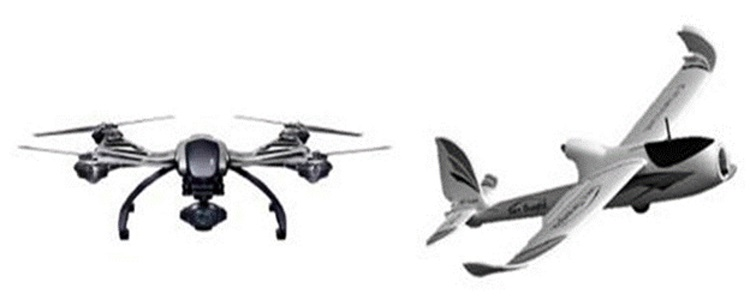
\includegraphics[width=10cm]{images/vant.jpg}
\centering
\end{figure}

%------------------------------------------------
\newpage
\subsection{Ala fija}

Es un término utilizado principalmente en la industria de la aviación para definir aeronaves que usan alas fijas y estáticas en combinación con la resistencia aerodinámica delantera para generar sustentación (la sustentación es la fuerza, de dirección perpendicular a la de la velocidad de la corriente incidente, generada sobre un cuerpo que se desplaza a través de un fluido). Ejemplos de este tipo de aeronaves son los aviones tradicionales, las cometas, y diferentes tipos de planeadores como parapentes. Incluso un simple avión de papel puede definirse como un sistema de ala fija.\\

\begin{figure}[h]
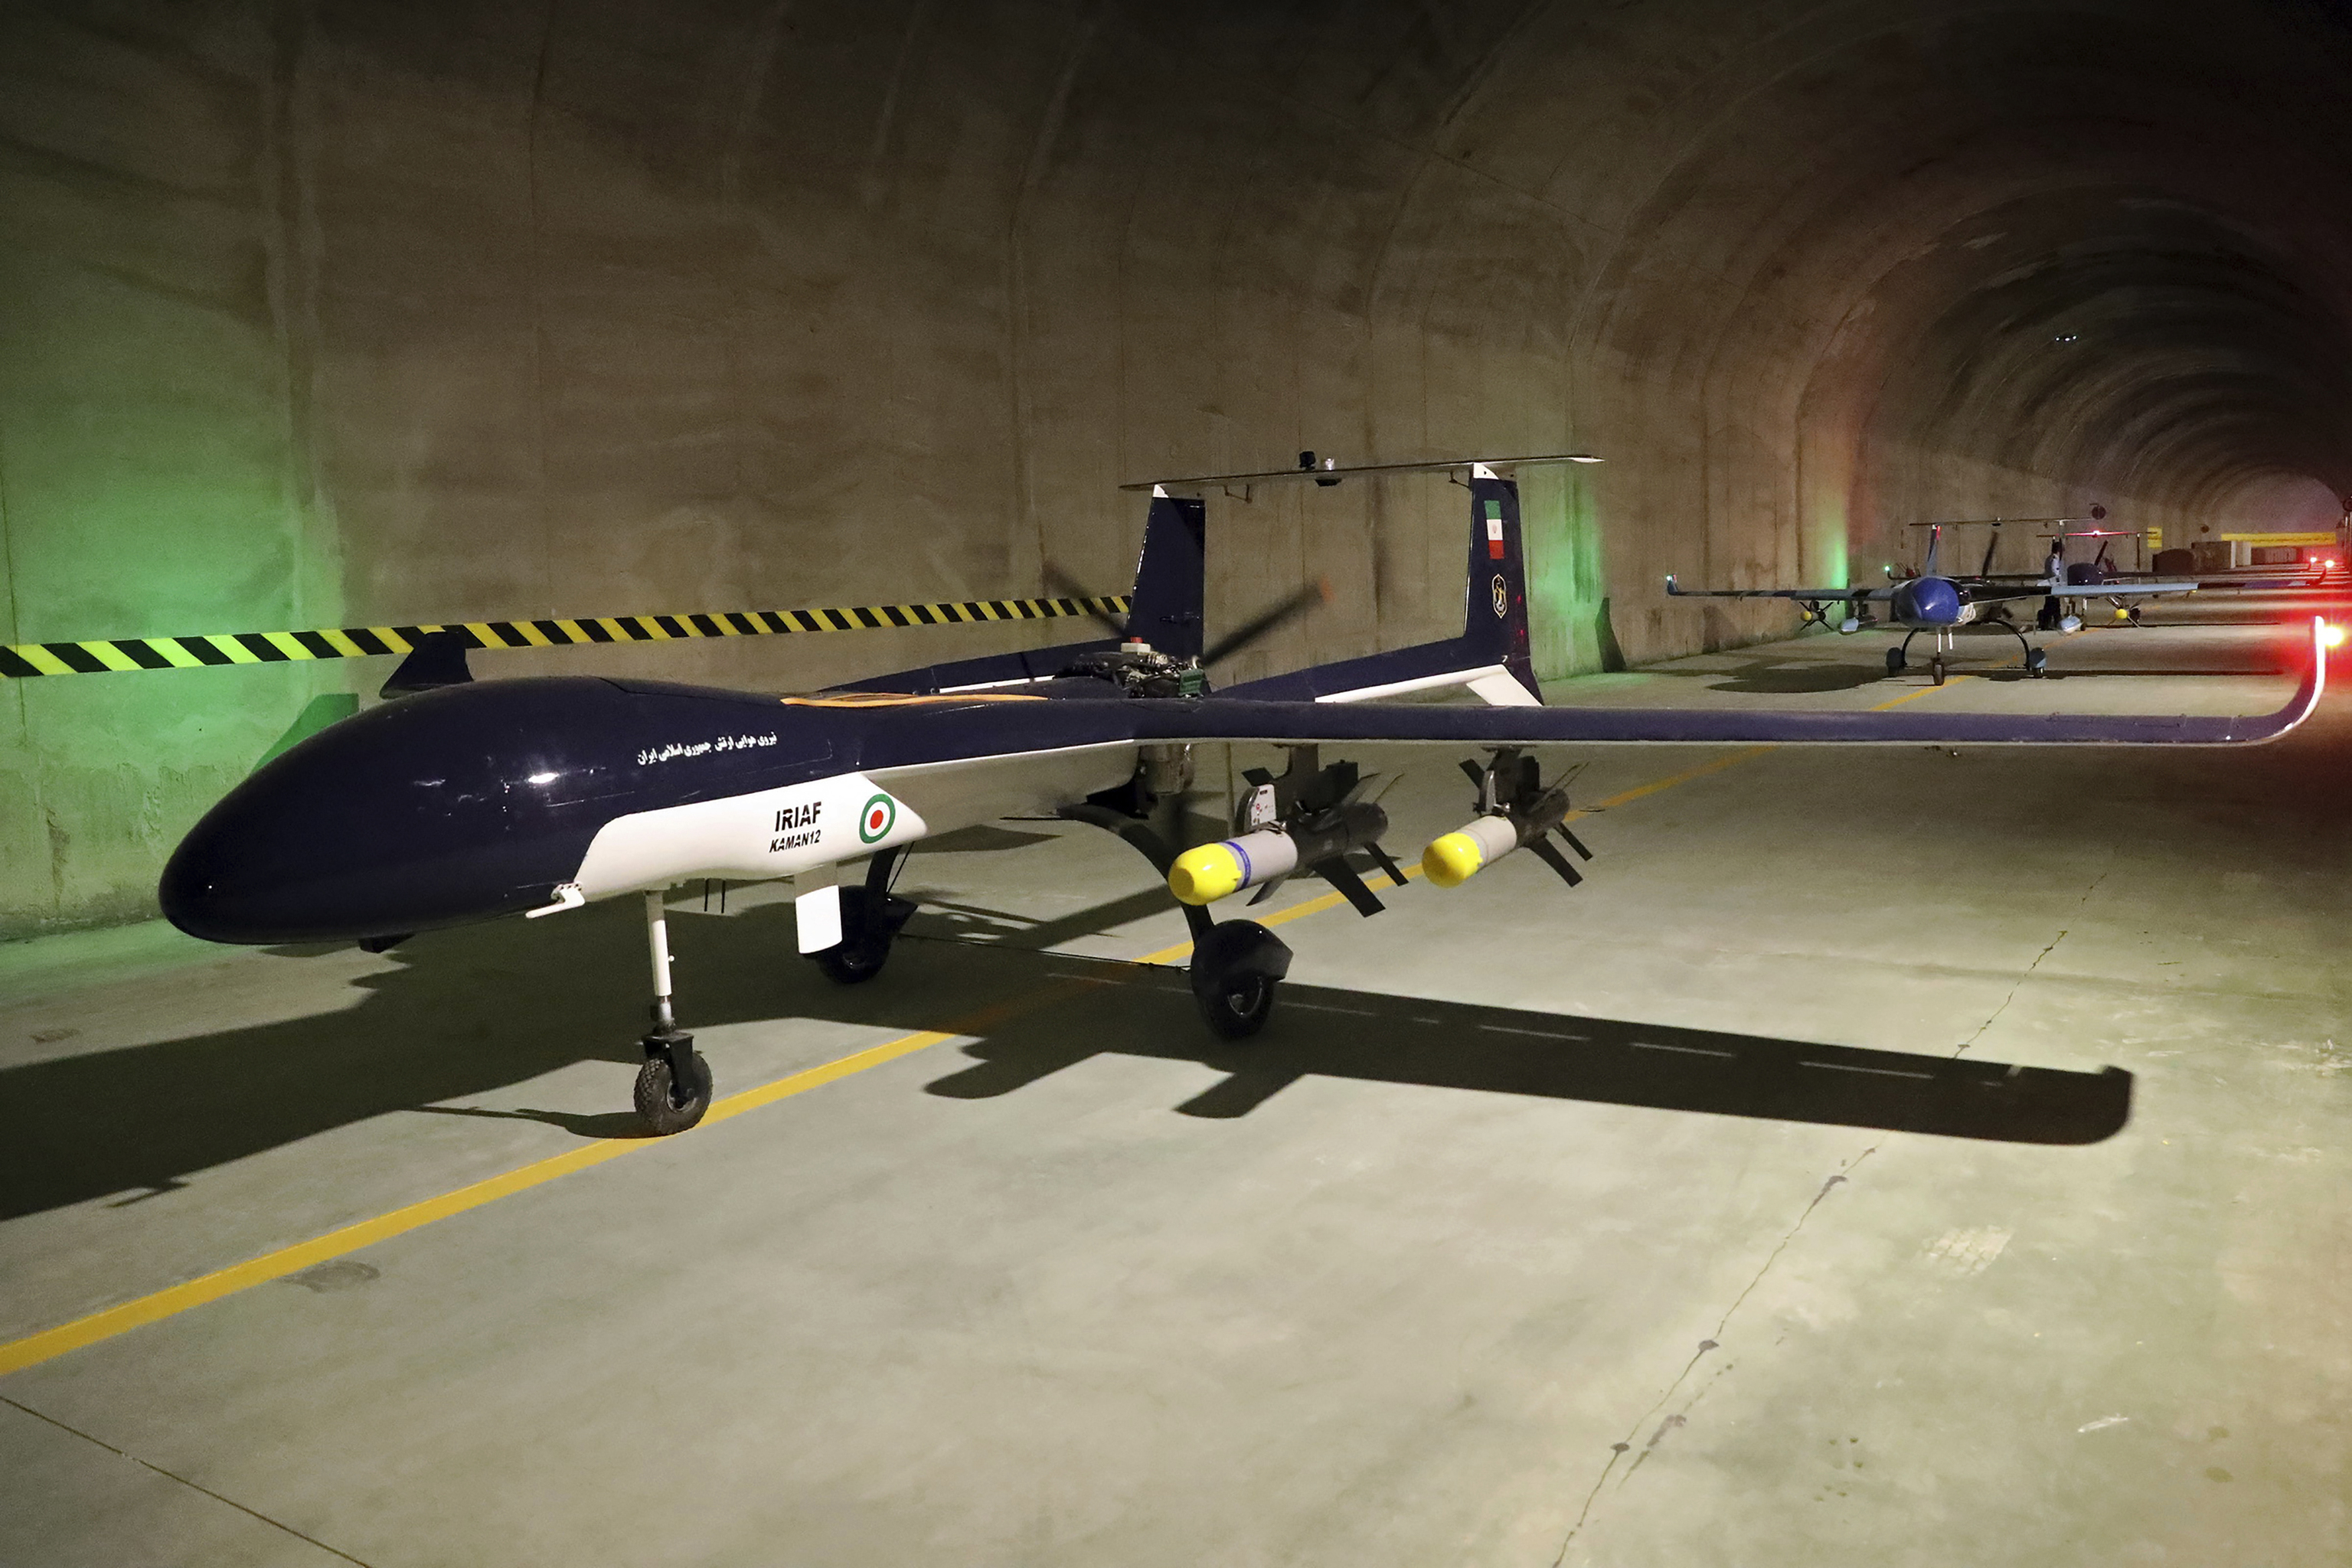
\includegraphics[width=10cm]{images/drone_alafija.jpg}
\centering
\end{figure}

%\begin{enumerate}
%\item Rango de funcionamiento:\\
%  Los drones de ala fija son la opción instintiva de los topógrafos que tradicionalmente han venido confiando en aeronaves tripuladas o imágenes por satélite para recopilar datos.\\
  
%  Eso suele deberse a la envergadura de la tarea en cuestión. Por ejemplo, los profesionales del campo y del sector petrolífero y gasístico probablemente opten por drones de ala fija porque comparten características ventajosas con las aeronaves tripuladas: rango de funcionamiento, velocidad de vuelo y autonomía de vuelo.\\
  
%  Al igual que los aviones normales, los drones de ala fija generan con sus alas una fuerza de sustentación. Esto quiere decir que, a diferencia de los drones multirrotor, no consumen grandes cantidades de energía para mantenerse en el aire y, en consecuencia, vuelan con más eficiencia.\\
  
%  \begin{figure}[h]
%    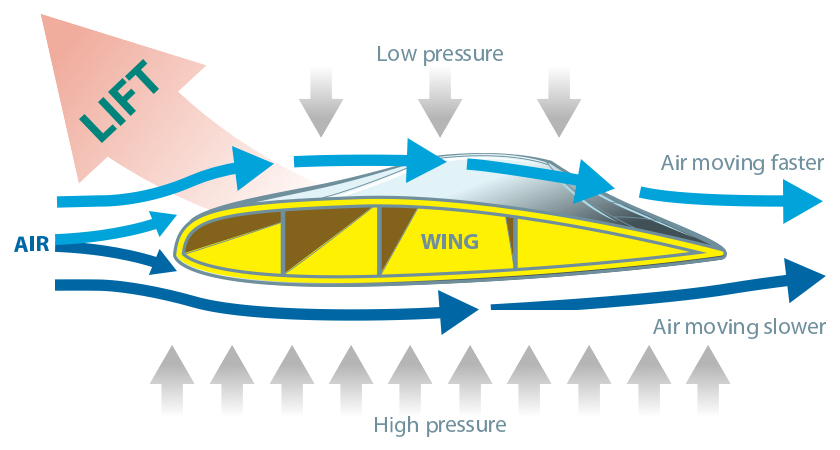
\includegraphics[width=10cm]{images/alafija.jpg}
%    \centering
%  \end{figure}
  
%\item Estabilidad en vientos:\\
%  El uso de drones de ala fija también puede comportar ventajas situacionales. Para empezar, los modelos de ala fija tienden a ser más aerodinámicos que las alternativas multirrotor y, en consecuencia, pueden soportar vientos de mayor intensidad. Además, debido al diseño tienen más facilidad para aterrizar sin sufrir desperfectos en caso de pérdida de potencia. Aunque, como veremos más adelante, esta característica también tiene sus inconvenientes.
  
%\item Autonomía de vuelo:\\
%  Se podría decir que la autonomía de vuelo que alcanzan los drones de ala fija es su ventaja más importante; la mayoría de los modelos son capaces de mantenerse en al aire más de una hora con una sola batería. Esta característica reduce los tiempos de inactividad operativas e implica que muchas tareas topográficas se puedan completar de una vez.
  
%\end{enumerate}

%------------------------------------------------

\subsection{Drones con rotor único}

Un dron con rotor único es un tipo de VANT (Vehículo Aéreo No Tripulado) que utiliza un solo rotor principal para generar la sustentación y el control en el aire. Este rotor único se encuentra ubicado verticalmente en el centro del dron y está conectado a un motor que lo hace girar a alta velocidad.\\

Este tipo de dron también es conocido como helicóptero no tripulado, es capaz de realizar vuelos estacionarios, despegues y aterrizajes verticales, y maniobras en diferentes direcciones. El control del vuelo se logra ajustando la velocidad y el ángulo de inclinación del rotor principal.\\

Los drones con rotor único suelen ser más ligeros y más eficientes energéticamente que los drones con múltiples rotores. Sin embargo también presentan desventajas como menor estabilidad debido a la ausencia de rotores adicionales.

\begin{figure}[h]
  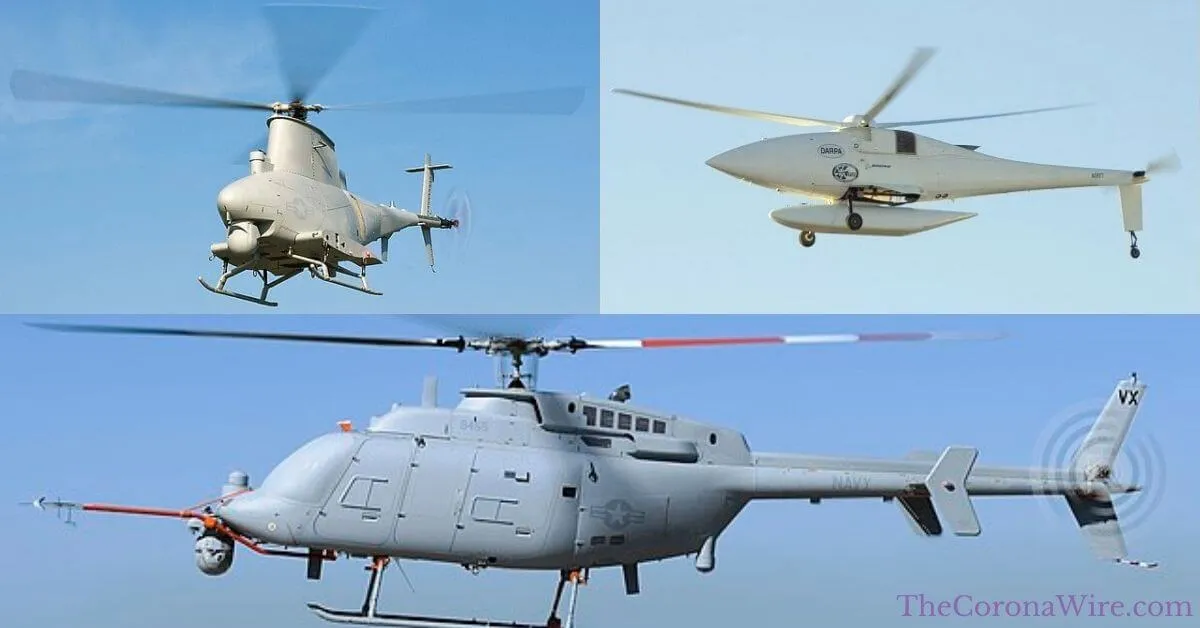
\includegraphics[width=10cm]{images/single_rotor.jpg}
  \centering
\end{figure}


\subsection{Drones Multi-rotor}

Un dron con múltiples rotores, también conocido como cuadricóptero (con cuatro rotores), hexacóptero (con seis rotores) o octocóptero (con ocho rotores), es un tipo de VANT (Vehículo Aéreo No Tripulado) que utiliza varios rotores para generar la sustentación y el control en el aire. Estos drones están equipados con varios rotores dispuestos de manera simétrica alrededor de su estructura. Cada rotor está conectado a un motor independiente y puede girar a diferentes velocidades y direcciones. Esta configuración permite que el dron ajuste individualmente la velocidad de cada rotor para controlar el ascenso, descenso, avance, retroceso, giro y desplazamiento lateral.\\

\begin{figure}[h]
  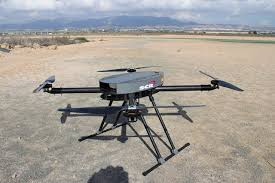
\includegraphics[width=8cm]{images/multi_rotor.jpg}
  \centering
\end{figure}

\subsection{Drones Híbridos}

Un dron híbrido es un tipo de VANT (Vehículo Aéreo No Tripulado) que combina características de los drones de ala fija y los drones de rotor múltiple. Estos drones están diseñados para tener la capacidad de volar tanto en modo de ala fija como en modo de rotor múltiple, lo que les brinda una mayor versatilidad y eficiencia en diferentes escenarios de vuelo.\\

En el modo de ala fija, el dron híbrido utiliza alas fijas similares a las de un avión. Estas alas generan la mayor parte de la sustentación y permiten vuelos de mayor alcance y eficiencia en términos de consumo de energía. El dron se impulsa hacia adelante mediante un motor o una hélice ubicada en el frente de la aeronave. Durante el vuelo en modo de ala fija, los rotores pueden estar inactivos o plegados para reducir la resistencia aerodinámica. Cuando se requiere un vuelo vertical o maniobras de vuelo más precisas, el dron híbrido puede cambiar al modo de rotor múltiple. En este modo, los rotores múltiples ubicados en la parte superior de la aeronave se activan y proporcionan la sustentación necesaria para despegues y aterrizajes verticales, así como para vuelos estacionarios. Los rotores también permiten un mayor control y maniobrabilidad en el aire.\\

\begin{figure}[h]
  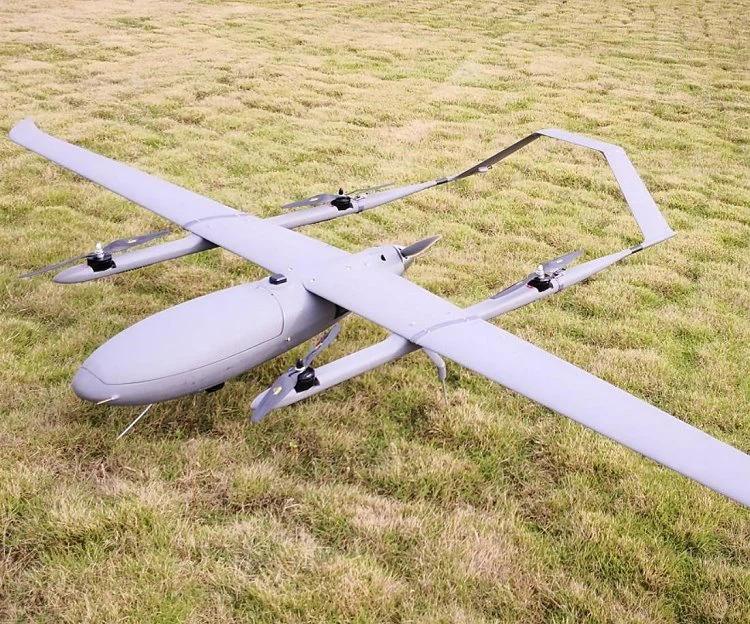
\includegraphics[width=7cm]{images/hybrid_drone.jpg}
  \centering
\end{figure}

\begin{sidewaystable}[h!]
  
  \begin{center}
    \begin{tabular}{| l | l | p{5cm} | p{5cm} | p{5cm} |}
      \hline
      TIPO & Sustentación & Ventajas & Desventajas & Aplicaciones \\ \hline
      Ala fija & Alas & Eficiencia en vuelos de larga distancia. Puede volar a gran altitud. & Espacio para despegue y aterrizaje. & Cartografía, monitoreo agrícola, vigilancia, inspeción \\ \hline
      Rotor único & Rotor & Estabilidad en vuelo & Menor autonomía en comparación con drones de ala fija & Fotografía, videografía, inspecciones \\ \hline
      Multiple Rotor & Rotor & Mayor estabilidad y capacidad de carga & Complejidad y costo en comparación con otros tipos & Fotografía, videografía, inspecciones \\ \hline
      Hibrido & Rotor y Ala & Versatilidad en diferentes modos de vuelo & Mayor complejidad de diseño y operación & Fotografía, inspecciones industriales \\
      \hline
    \end{tabular}
  \end{center}
  
\end{sidewaystable}

\end{document}
